\chapter{Results}
\label{ch:results}

\section{Input resolution}
\label{sec:resolution}

\subsection{Accuracy does not discriminate}

\begin{table}[htbp]
\centering
\begin{tabular}{lcccc}
\toprule
Input size & Val.\ accuracy & Std.\ dev. & Observed range & Epochs \\
\midrule
224\,px & 0.9854 & 0.0007 & 0.9847--0.9861 & 22.7 \\
112\,px & 0.9800 & 0.0035 & 0.9777--0.9840 & 17.3 \\
64\,px  & 0.9814 & 0.0011 & 0.9805--0.9826 & 24.7 \\
\bottomrule
\end{tabular}
\caption{Validation accuracy by input resolution, mean and standard deviation
over three seeds.}
\label{tab:resolution-accuracy}
\end{table}

The ordering in Table~\ref{tab:resolution-accuracy} is not monotonic --- 64\,px
outperforms 112\,px --- and a genuine resolution effect would produce monotonic
degradation. The arithmetic agrees: $0.9854$ corresponds to $21.0$ errors out of
$1\,435$ validation samples and $0.9814$ to $26.6$, a gap of $5.6$ samples,
against a 95\,\% Wilson interval on a single measurement of $\pm 0.7$ percentage
points. The four classes survive an elevenfold reduction in pixel count,
consistent with their being distinguished by coarse morphology rather than fine
texture.

Per-class recall is directional but small. Violin\_Mode degrades most from
224\,px to 64\,px, by $1.00$ percentage points, which is the direction predicted
from morphology since narrow spectral lines are the structure most vulnerable to
downsampling --- but the magnitude is $3.6$ samples out of $365$, inside the
confidence interval of a single measurement. Extremely\_Loud degrades more at
112\,px than at 64\,px, a second non-monotonicity. \textbf{No class collapses at
reduced resolution.}

\subsection{Network health does discriminate}

Since accuracy is uninformative, the resolution was decided on the internal state
of the network. For each hidden layer, the mean firing rate of every individual
neuron is accumulated across the validation partition. A rate below $0.01$
identifies a \emph{dead} neuron, above $0.80$ a \emph{saturated} one. Both are
pathological in different ways: dead neurons represent wasted capacity and,
being permanently silent, cannot appear in any explanation; saturated neurons
carry almost no information, a nearly-always-firing binary unit having minimal
entropy, while consuming the maximum possible energy.

\begin{table}[htbp]
\centering
\begin{tabular}{lcccc}
\toprule
Input size & Layer 1 & Layer 2 & Layer 3 & Layer 4 \\
\midrule
224\,px & $12.1 \pm 3.3$ & $16.6 \pm 4.9$ & $12.6 \pm 2.3$ & $\mathbf{36.3 \pm 4.0}$ \\
112\,px & $17.8 \pm 3.4$ & $11.8 \pm 0.8$ & $13.0 \pm 1.0$ & $\mathbf{23.6 \pm 2.9}$ \\
64\,px  & $16.4 \pm 4.8$ & $11.2 \pm 2.3$ & $11.7 \pm 2.3$ & $\mathbf{19.5 \pm 1.5}$ \\
\bottomrule
\end{tabular}
\caption{Percentage of dead neurons by layer and resolution, mean $\pm$ standard
deviation over three seeds, on validation.}
\label{tab:dead}
\end{table}

Layer 4 is the only layer that responds to resolution, and it responds on two
measures at once: the dead fraction falls monotonically from $36.3$\,\% to
$19.5$\,\%, while the median per-neuron firing rate rises from $0.0399$ to
$0.1499$. These were the two competing explanations for the higher mean activity
observed at lower resolution --- more neurons participating, or the same neurons
firing harder --- and both occur. Saturation does not increase to compensate:
neurons above $0.80$ remain below $2.5$\,\% in layer 4 at every resolution.

\textbf{The interpretation is spatial redundancy, not a cured pathology.} Layer 4
contains $25\,088$ neurons at 224\,px and $6\,272$ at 112\,px, so in absolute
terms the number of \emph{live} neurons falls from roughly $15\,970$ to $4\,789$.
Reducing the resolution does not increase usable capacity; it reduces capacity
while preferentially discarding units that were contributing nothing. At 224\,px
the deepest layer views a $14 \times 14$ map derived from a largely empty
spectrogram, and a third of its units never encounter signal.

\subsection{Decision: 112 pixels}

Most of the benefit comes from the first halving: 224 to 112\,px recovers $12.7$
percentage points of dead fraction, the further move to 64\,px only $4.1$ more.
Membrane state at 8 bits falls from 368\,KiB to 92\,KiB, bringing the full
inference state within the SRAM budget of the target class of devices.

The decisive argument against 64\,px is the spatial resolution of the
explanations themselves. SAM maps are computed on layer activations, whose side
lengths are 56, 28, 14 and 7 at 112\,px but 32, 16, 8 and 4 at 64\,px. A
$4 \times 4$ map contains sixteen values, on which centre-of-mass, top-$K$
intersection-over-union and structural similarity are all meaningless. Since the
contribution of this thesis is the fidelity of explanations rather than of
predictions, a configuration in which the measured object is degenerate in one
layer cannot be accepted whatever it saves in compute.

\section{Hyperparameters and the full-precision reference}
\label{sec:hyperparameters}

The constrained search selected \textbf{$\beta = 0.75$, $T = 8$, learning rate
$1.047 \times 10^{-4}$} at a best validation accuracy of $0.9847$ within the
15-epoch budget.

\textbf{The constraint on $\beta$ is justified empirically, not only by
argument.} An unconstrained search over $\beta \in (0,1)$ selects $0.4148$, whose
nearest admissible neighbours are $0.25$ and $0.5$. The constrained search
selects $0.75$. Rounding the unconstrained optimum after the fact --- the
alternative to constraining the space --- would therefore have produced a
configuration that is both inferior and never validated.

All four values were sampled; the search allocated 40\,\% of trials to $0.75$ and
10\,\% to $0.875$, which is itself the surrogate model's judgement after early
exploration. Among trials surviving at least three epochs, $0.75$ leads on both
the best ($0.9847$) and the median ($0.9763$) validation accuracy, while $0.875$
trails on both and was pruned in all three of its trials.

\textbf{$T = 8$ is an optimum at the imposed ceiling} and is reported as such:
the search was forbidden from exploring $T > 8$. The mitigating evidence is that
an unconstrained search with range up to 15 selected $T = 7$, so the preference
for long integration windows is mild.

\subsection{$\beta$ improves the measurement instrument}

Holding resolution and partition fixed and changing only $\beta$ from $0.4148$ to
$0.75$, the layer-4 dead fraction is \emph{unchanged} at $23.6$\,\%. $\beta$ does
not affect the dead fraction; resolution does. This strengthens the reading of
Section~\ref{sec:resolution}: the deep-layer problem is spatial redundancy rather
than a dynamical pathology curable by a better decay constant.

What $\beta$ does change is saturation, by an order of magnitude and most where
it matters. Neurons above $0.80$ fall from $9.3 / 3.5 / 2.7 / 1.8$\,\% across the
four layers to $4.7 / 0.22 / 0.06 / 0.14$\,\%. The layer-2 figure is the
consequential one, because a saturated neuron accumulates the maximum possible
contribution score on every image and therefore contributes a constant,
non-discriminative floor to every SAM map. \textbf{Selecting $\beta$ on
validation accuracy alone happened to reduce that contamination by a factor of
sixteen at the reference layer.}

\subsection{Three-seed reference}

\begin{table}[htbp]
\centering
\begin{tabular}{lcc}
\toprule
Quantity & Mean & Std \\
\midrule
Validation accuracy & 0.9833 & 0.0014 \\
Epochs to early stop & 21.0 & 1.7 \\
Recall, Blip & 0.9915 & 0.0028 \\
Recall, Extremely\_Loud & 0.9855 & 0.0000 \\
Recall, Scattered\_Light & 0.9839 & 0.0027 \\
Recall, Violin\_Mode & 0.9726 & 0.0099 \\
\bottomrule
\end{tabular}
\caption{Full-precision reference at 112\,px, $\beta = 0.75$, $T = 8$, over three
seeds on validation.}
\label{tab:fp32}
\end{table}

The reference is statistically indistinguishable from the 224\,px configuration
($0.9854$): three samples out of $1\,435$ separate them, against a four-sample
spread across seeds. \textbf{Reducing the pixel count by a factor of four, and
constraining $\beta$ and $T$ to hardware-realizable values, costs no measurable
accuracy.}

\textbf{Accuracy is reproducible; internal dynamics are not.} At fixed accuracy
the mean firing rate of layer 1 varies by a factor of $2.6$ across seeds, and the
coefficient of variation falls monotonically with depth: $46.9$\,\% at layer 1,
$28.6$\,\% at layer 2, $15.3$\,\% at layer 3, $9.5$\,\% at layer 4. The regime is
established within the first epoch and persists, indicating that initialization
selects the firing regime and training does not subsequently equalize it. A
measurement taken during the resolution study puts the effect in the units of
the closest work: the Wasserstein-1 distance between the per-layer firing-rate
profiles of two full-precision models differing only in seed is $0.039$, inside
the range of Earth Mover's Distances that Smith et al.~\cite{smith2026} report
\emph{between full-precision and quantized} models. This is the observation that
motivates Section~\ref{sec:calibration}.

\section{Physical validation of the dynamics}
\label{sec:physical}

At the adopted configuration the confusion matrix diagonal reads
$0.99 / 0.99 / 0.98 / 0.97$, consistent with Table~\ref{tab:fp32}; the only
non-negligible errors are on Violin\_Mode, the class that in the tabular domain
partially overlaps both Blip and Scattered\_Light (Figure~\ref{fig:confusion}).

\begin{figure}[htbp]
\centering
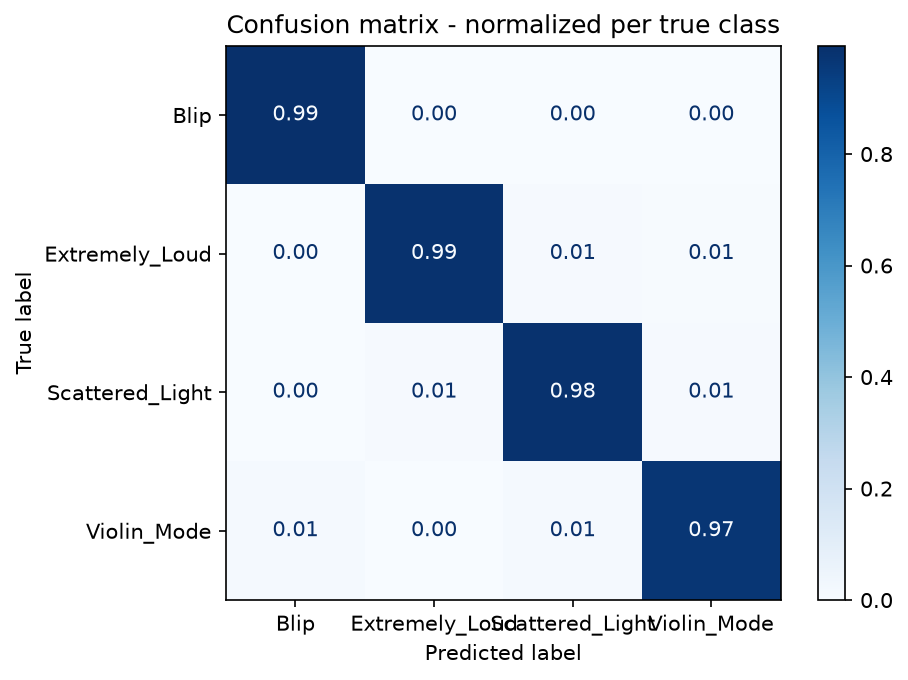
\includegraphics[width=0.6\linewidth]{confusion_matrix.png}
\caption{Confusion matrix of the reference checkpoint (seed 1234) on validation,
normalized per true class.}
\label{fig:confusion}
\end{figure}

The dead fraction is $16.1 / 12.6 / 11.3 / 22.8$\,\% across the four layers, and
\textbf{no neuron in any layer exceeds the saturation threshold}, a consequence
of $\beta = 0.75$ (Figure~\ref{fig:firing}). These figures reproduce those of Section~\ref{sec:resolution}
exactly for the same seed, computed through an independent code path, which is a
free verification of both.

One feature deserves note: the layer-1 distribution is \textbf{bimodal}, with a
secondary population near a firing rate of $0.65$--$0.75$ that has no counterpart
in the deeper layers. A high-activity subpopulation therefore exists in the first
layer only, which may be related to its being the layer with the largest
coefficient of variation across seeds.

\begin{figure}[htbp]
\centering
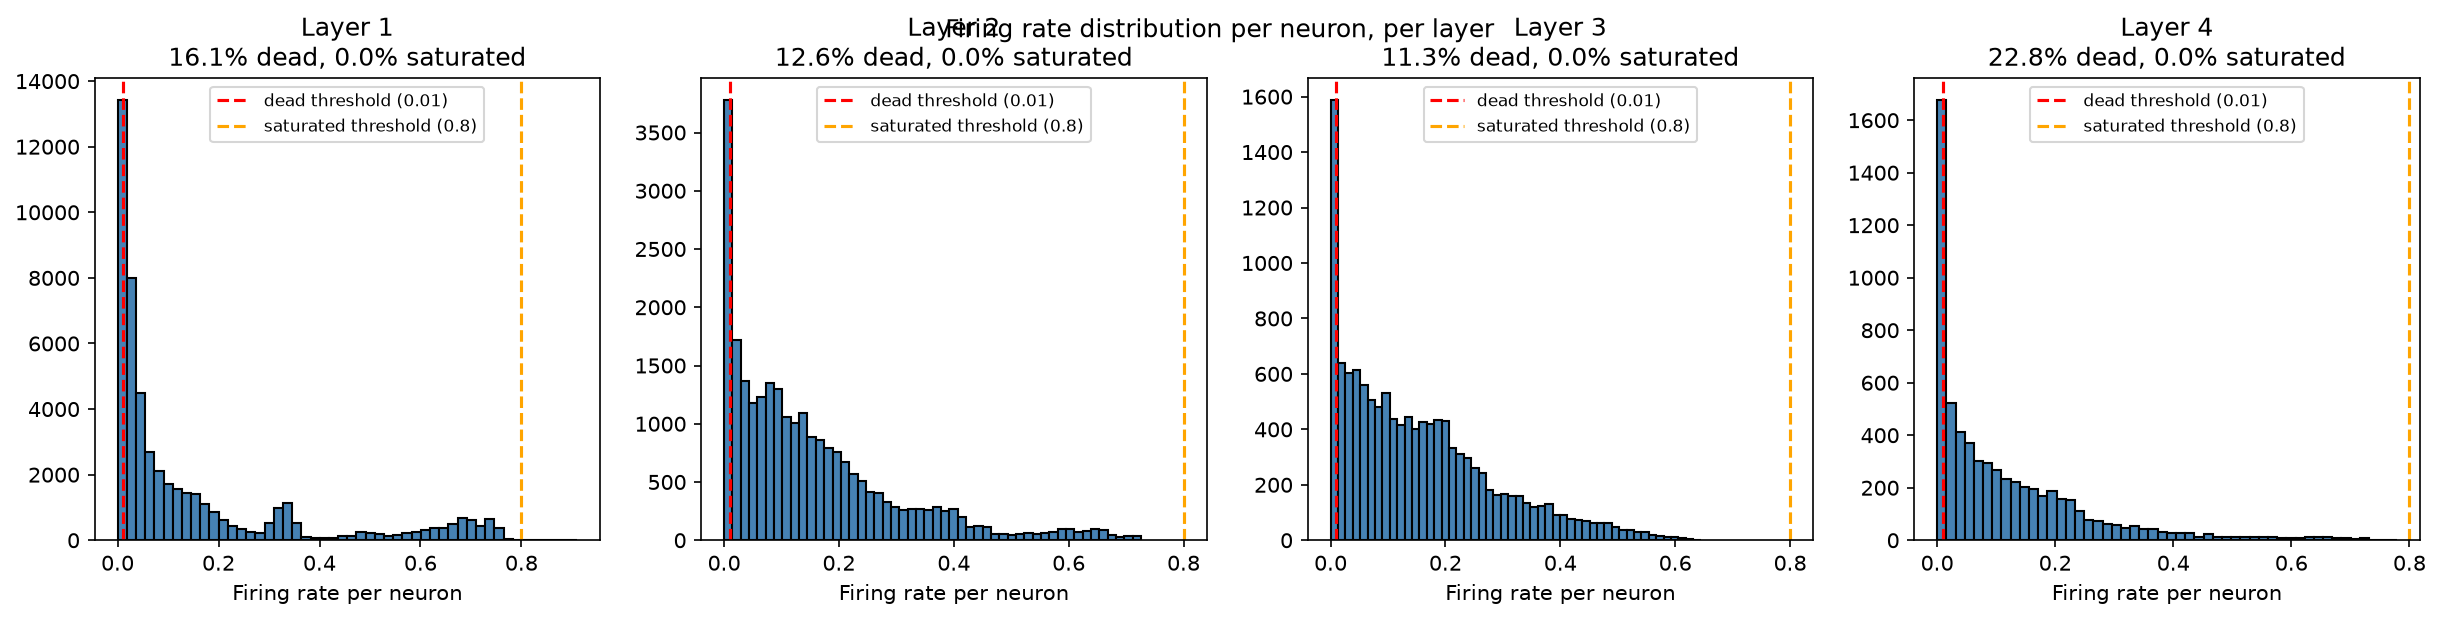
\includegraphics[width=\linewidth]{firing_rate_distributions.png}
\caption{Distribution of per-neuron firing rates in the four hidden layers, on
validation, with the dead ($0.01$) and saturation ($0.80$) thresholds.}
\label{fig:firing}
\end{figure}

The coefficient of variation of inter-spike intervals concentrates between $0.35$
and $0.45$ in all four layers. Firing is regular rather than Poisson-like, which
is the expected outcome under constant direct encoding: since the input does not
vary over time, any irregularity observed is generated entirely by the membrane
dynamics and by interaction between layers. This is evidence about internal
dynamics, not a claim of biological realism. With $T = 8$ a neuron can produce at
most seven intervals, so the five-interval threshold used for the estimate is
close to the ceiling, which is why the accumulation runs over the whole partition
rather than a single image. Between 184 and 196 of the 200 sampled neurons per
layer met the threshold (Figure~\ref{fig:cvisi}).

\begin{figure}[htbp]
\centering
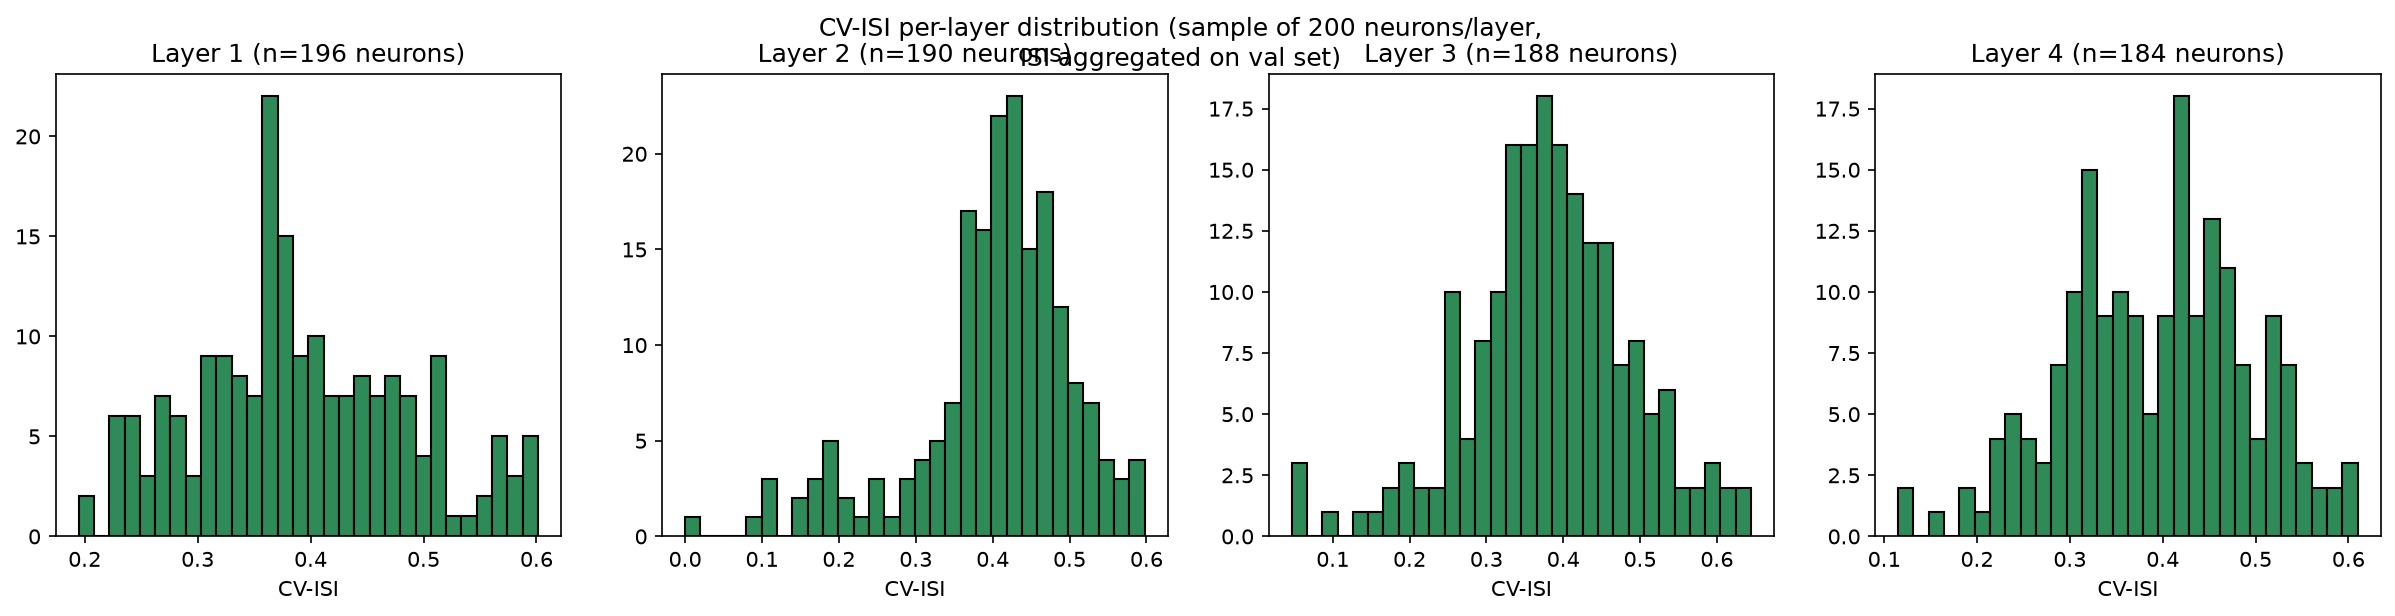
\includegraphics[width=\linewidth]{cv_isi_distributions.png}
\caption{CV of inter-spike intervals for 200 sampled neurons per layer,
accumulated over the validation partition.}
\label{fig:cvisi}
\end{figure}

\section{What the explanations show}
\label{sec:sam-results}

Figure~\ref{fig:sam-steps} shows the SAM sequence of a single Blip at the
reference layer. The map is zero at $t = 0$ by definition and builds up over
the first steps as spike histories accumulate; from the third step onward the
attended region is the vertical stroke of the glitch.

\begin{figure}[htbp]
\centering
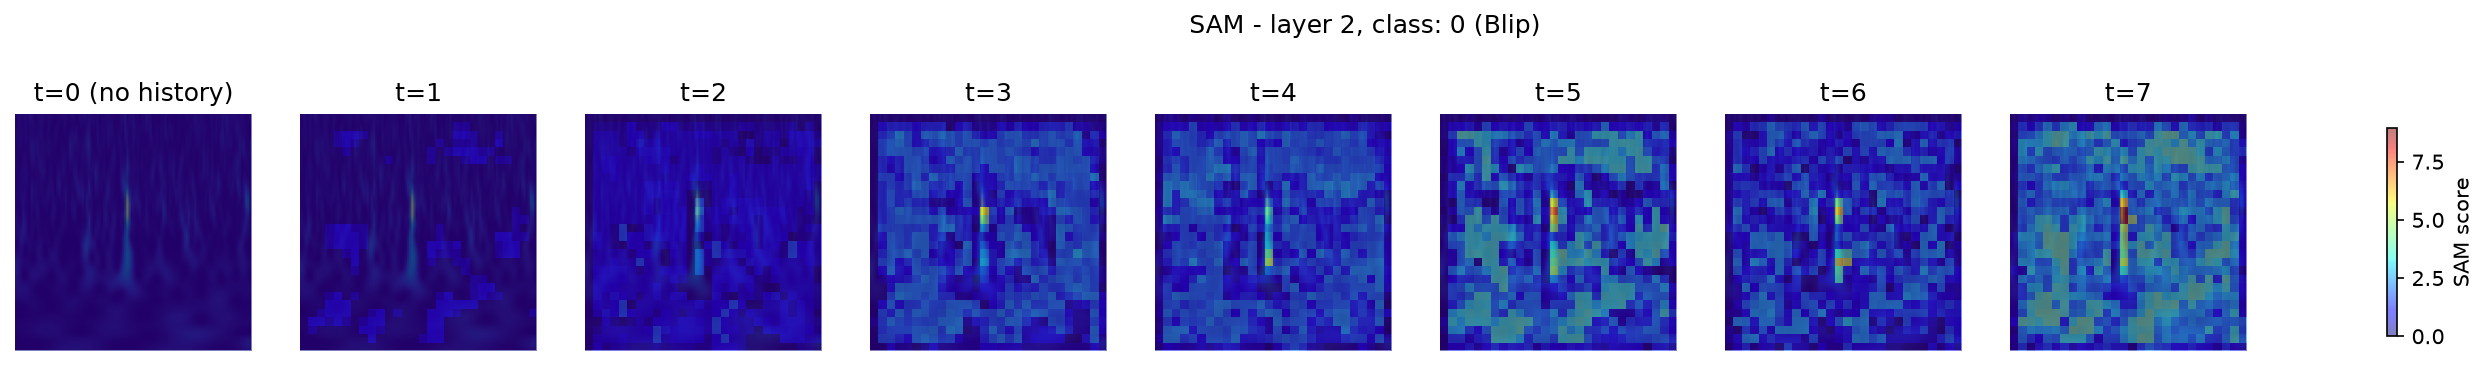
\includegraphics[width=\linewidth]{sam_visualization.png}
\caption{SAM at layer 2 for one Blip, one panel per time step, on a shared
colour scale.}
\label{fig:sam-steps}
\end{figure}

The class statistics (Figure~\ref{fig:sam-class}) show four recognizably
different attention patterns, each matching the morphology of its class. For
Blip the mean map concentrates on the narrow vertical stroke and so does the
variability, which is the stroke shifting slightly between instances. For
Extremely\_Loud the attended region is large and saturated, covering the lower
and central part of the spectrogram. For Scattered\_Light the attention lies on
a horizontal band at low frequency. Violin\_Mode produces the weakest and most
diffuse mean map, with variability concentrated in a few localized spots along
the line structure; it is also the class with the lowest recall, and the one
whose explanations prove most sensitive in every test below.

\begin{figure}[htbp]
\centering
\includegraphics[width=0.9\linewidth]{sam_class_stats.png}
\caption{SAM statistics per class at layer 2, 25 validation images per class:
mean (top), standard deviation (middle) and coefficient of variation (bottom,
truncated at the 95th percentile). Mean and standard deviation share a colour
scale across classes.}
\label{fig:sam-class}
\end{figure}

Across depth (Figure~\ref{fig:sam-layers}) the progression is the expected one,
from fine localization in the early layers to coarse localization in the deep
ones, with maps of side 56, 28, 14 and 7. At layer 4 a $7 \times 7$ map leaves
only 49 positions, too few for a top-20\,\% overlap or a structural comparison
to be meaningful, while layer 2 still resolves the morphology of every class.

\todo{Confirm (or replace) this as the reason for choosing layer 2 as the
reference layer; the progress report records the choice but not its
justification.}

\begin{figure}[htbp]
\centering
\begin{subfigure}{0.49\linewidth}
  \includegraphics[width=\linewidth]{sam_layer_Blip.png}
  \caption{Blip}
\end{subfigure}\hfill
\begin{subfigure}{0.49\linewidth}
  \includegraphics[width=\linewidth]{sam_layer_Extremely_Loud.png}
  \caption{Extremely\_Loud}
\end{subfigure}

\begin{subfigure}{0.49\linewidth}
  \includegraphics[width=\linewidth]{sam_layer_Scattered_Light.png}
  \caption{Scattered\_Light}
\end{subfigure}\hfill
\begin{subfigure}{0.49\linewidth}
  \includegraphics[width=\linewidth]{sam_layer_Violin_Mode.png}
  \caption{Violin\_Mode}
\end{subfigure}
\caption{SAM mean and standard deviation across the four hidden layers, 20
images per class, normalized by the channel count of each layer.}
\label{fig:sam-layers}
\end{figure}

\section{Fixing the explainer}

\subsection{Choice of the decay rate}
\label{sec:gamma}

SAM has one free parameter, and an explanation that changed qualitatively with an
arbitrary choice of $\gamma$ would not be trustworthy.

\textbf{$\gamma$ is the decay of a temporal kernel, so it must be evaluated on
the temporal axis.} Comparing maps averaged over time removes precisely the axis
on which $\gamma$ acts, and a high spatial correlation is then close to
guaranteed regardless of $\gamma$. Three quantities are therefore measured: the
spatial Pearson correlation between time-aggregated maps, retained for continuity
with the literature; the \emph{temporal centre of mass} of the SAM energy; and
the \emph{per-timestep correlation} against a reference $\gamma$.

Before a null result could be trusted, the instrument was checked analytically:
on a fully firing spike train with $T = 8$ the centre of mass moves from $4.86$
at $\gamma = 0.1$ to $4.02$ at $\gamma = 3.0$, so the metric does respond. A
second check comes free from the definition: at $t = 1$ the score is
$e^{-\gamma} S_0$, so changing $\gamma$ multiplies the map by a constant, and
Pearson correlation is affine-invariant. The measured per-timestep correlation at
$t = 1$ is exactly $1.000$ for every $\gamma$, as it must be.

\begin{table}[htbp]
\centering
\begin{tabular}{lcccc}
\toprule
Class & Spatial PCC, $\gamma$ 0.1 vs 3.0 & CoM at 0.1 & at 3.0 & Shift \\
\midrule
Extremely\_Loud & 0.9993 & 4.973 & 4.144 & 0.829 \\
Blip & 0.9890 & 5.192 & 4.339 & 0.853 \\
Scattered\_Light & 0.9758 & 5.271 & 4.352 & 0.919 \\
Violin\_Mode & 0.9598 & 5.260 & 4.327 & 0.933 \\
\bottomrule
\end{tabular}
\caption{$\gamma$ sensitivity at layer 2, mean over fifteen validation images per
class.}
\label{tab:gamma}
\end{table}

Two conclusions follow, and neither is the one the naive analysis would reach.

\textbf{The temporal shift is largely kernel arithmetic rather than explanation
structure.} The measured shift of $0.83$--$0.93$ steps matches what a
\emph{fully firing} spike train produces ($0.84$), whereas the layer-2 firing
rate is approximately $0.19$ and simulated random trains at that density shift by
only $0.26$ steps. SAM is therefore dominated by a minority of near-continuously
firing neurons, for which the centre of mass follows the exponential kernel. The
centre of mass against $\gamma$ is consequently \emph{not} a useful criterion for
selecting $\gamma$ --- though it remains valid as a divergence metric, where
models are compared at fixed $\gamma$ and the trivial component cancels, and it
now carries a reference scale.

\textbf{Sensitivity is strongly class-dependent.} In terms of $1 - \mathrm{PCC}$,
Violin\_Mode is 57 times more sensitive than Extremely\_Loud. The ordering
Violin\_Mode $>$ Scattered\_Light $>$ Blip $>$ Extremely\_Loud recurs identically
under the two unrelated interventions of Section~\ref{sec:calibration}.

Within $\gamma \in [0.3, 0.9]$ all per-timestep correlations remain above $0.98$
even in the worst class; only $\gamma = 3.0$ diverges appreciably.
\textbf{$\gamma = 0.5$ is adopted}, the value of the original
formulation~\cite{kim2021sam}, now supported by evidence on the axis $\gamma$
actually governs (Figure~\ref{fig:gamma}).

\begin{figure}[htbp]
\centering
\includegraphics[width=\linewidth]{gamma_Violin_Mode.png}
\caption{$\gamma$ sensitivity for Violin\_Mode, the most sensitive class, at
layer 2. The equivalent figures for the other three classes are in
Appendix~\ref{app:figures}.}
\label{fig:gamma}
\end{figure}

\subsection{Faithfulness}
\label{sec:faithfulness}

Robustness to $\gamma$ is necessary but not sufficient: a stable explanation can
be stably wrong. The deletion metric~\cite{petsiuk2018rise} removes pixels in
decreasing order of SAM score and records the confidence assigned to the class
predicted on the unmodified image, comparing against removal in random order.

Three implementation details govern interpretation. Deleted pixels are set to
zero \emph{in normalized space}, corresponding to the dataset mean rather than to
black, a neutral substrate that avoids injecting an artificial edge. The same map
is used for both orderings. And the ordering is computed once per image and
sliced progressively, so the masked sets are nested: what is removed at 50\,\%
stays removed at 55\,\%. Regenerating a random permutation at each fraction would
break nesting for the baseline while leaving it intact for SAM, making the two
curves incomparable.

\begin{table}[htbp]
\centering
\begin{tabular}{lccccl}
\toprule
Class & AUC-SAM & AUC-random & $\Delta$ & Relative & Reading \\
\midrule
Blip & 0.3119 & 0.4795 & $-0.1676$ & $-35.0$\,\% & faithful \\
Extremely\_Loud & 0.6121 & 0.8892 & $-0.2771$ & $-31.2$\,\% & faithful \\
Scattered\_Light & 0.3835 & 0.3650 & $+0.0185$ & $+5.1$\,\% & not separable \\
Violin\_Mode & 0.4528 & 0.4540 & $-0.0012$ & $-0.3$\,\% & indistinguishable \\
\bottomrule
\end{tabular}
\caption{Deletion metric by class, 15 validation images each. A faithful
explanation gives AUC-SAM below AUC-random, so a negative $\Delta$ is expected.}
\label{tab:deletion}
\end{table}

\begin{figure}[htbp]
\centering
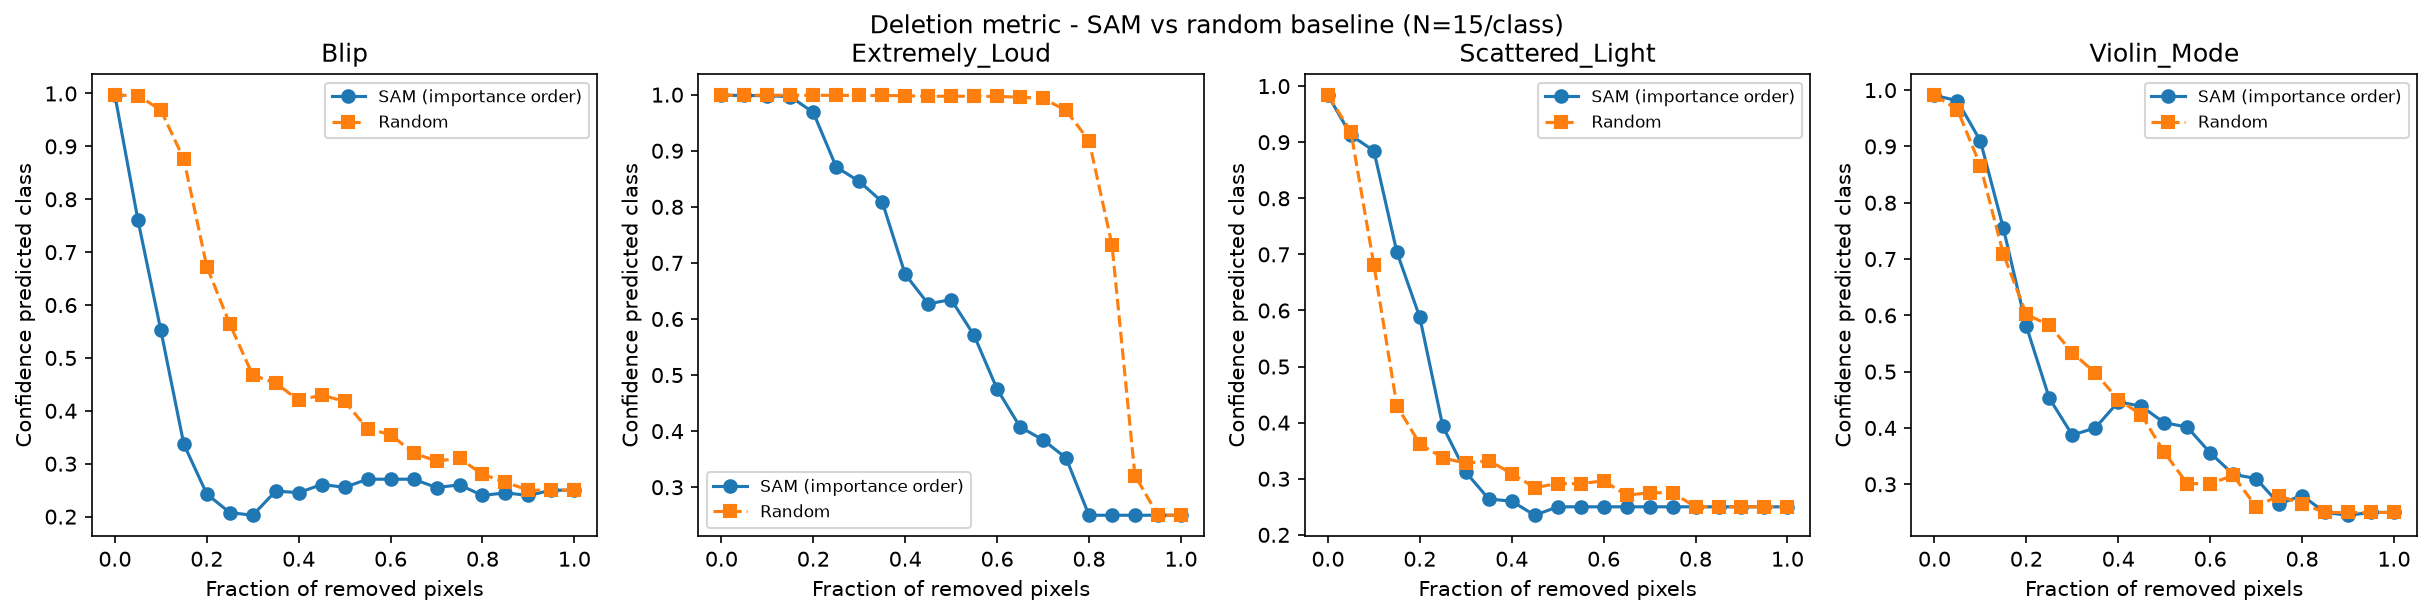
\includegraphics[width=\linewidth]{deletion_metric.png}
\caption{Deletion curves, SAM order against random order, 15 validation images
per class.}
\label{fig:deletion}
\end{figure}

The metric separates SAM from the baseline on two classes and not on the other
two, and the split is systematic. Blip and Extremely\_Loud show reductions of
$35$ and $31$\,\% in area. Violin\_Mode is within $0.3$\,\% of the baseline.
Scattered\_Light is nominally inverted, but at $+5.1$\,\% the magnitude is one
sixth of the two positive effects, so it is better described as an absence of
separation with a slight drift in the wrong direction than as a genuine reversal.

The pattern follows the spatial geometry of the classes rather than any property
of SAM. Blip is a compact vertical line and Extremely\_Loud a dominant saturated
structure, so removing the high-scoring region removes the defining evidence.
Scattered\_Light is an extended horizontal band and Violin\_Mode a set of thin
distributed lines: random deletion fragments the pattern across the whole image,
whereas SAM-guided deletion concentrates removal in one region and leaves the
rest --- which still carries sufficient evidence --- intact. This is a known
limitation of deletion-based tests, which penalize explanations of spatially
extended features, and it is reported rather than suppressed.

Two controls confirm the measurement itself. All curves converge to
approximately $0.25$ at full deletion, which is chance for four classes. And the
Extremely\_Loud random baseline remaining at $0.8892$, the highest of the four,
is independent confirmation of that class's behaviour below: its evidence is
distributed across the whole image, which is why no localized removal registers.

\section{Calibrating the divergence metrics}
\label{sec:calibration}

The metrics used to compare two explanations return numbers between zero and one
whatever is fed to them. Three questions must be answered before any quantization
result can be interpreted: what they report when nothing has changed, when
something negligible has changed, and when everything has changed.

All measurements use fifteen validation images per class at layer 2 with
$\gamma = 0.5$, on the three checkpoints of Table~\ref{tab:fp32}.

\subsection{Verification of the instrument}

Comparing a checkpoint against itself returns $\mathrm{PCC} = 1$,
$\mathrm{IoU} = 1$ and a centre-of-mass difference of $0$ to within $10^{-9}$,
confirming that the metrics and the image pairing are correct. Two separate calls
to the sampling routine return bit-identical image tensors, confirming that every
model sees the same data. A second forward pass of the same model reproduces the
maps exactly, confirming that the network is deterministic in evaluation mode and
that the cross-model differences below are not run-to-run noise.

\subsection{Two independent solutions}

\begin{table}[htbp]
\centering
\begin{tabular}{lccccc}
\toprule
Class & PCC mean & worst & IoU mean & worst & CoM diff, max \\
\midrule
Extremely\_Loud & 0.917 & 0.869 & 0.520 & 0.460 & 0.076 \\
Violin\_Mode & 0.844 & 0.816 & 0.597 & 0.543 & 0.115 \\
Blip & 0.612 & 0.336 & 0.593 & 0.503 & 0.083 \\
Scattered\_Light & 0.477 & \textbf{0.153} & 0.376 & 0.234 & 0.104 \\
\bottomrule
\end{tabular}
\caption{Divergence between full-precision models differing only in seed, over
the three seed pairs. Chance-level IoU at $k = 0.20$ is $0.111$.}
\label{tab:seeds}
\end{table}

\textbf{The spatial metrics collapse.} Two models agreeing to within one
validation sample in accuracy produce maps correlating at $0.153$ on
Scattered\_Light, with a top-20\,\% overlap of $0.234$ against a chance level of
$0.111$. For comparison, a thirtyfold change in $\gamma$ reduces the correlation
only to $0.960$: initialization variance is 21 times larger than that effect.

The per-image distribution rules out an outlier explanation. On Blip the fifteen
per-image correlations run from $0.147$ to $0.768$ with a median of $0.282$, and
twelve of the fifteen fall below $0.35$. The disagreement is uniform across
samples.

The mechanism is not a defect of the metric. Networks trained from different
initializations learn functionally equivalent but \textbf{permuted}
representations, so a pixel-wise comparison between them compares arbitrary
assignments of channels to positions rather than information content. This is why
the result is a bound on cross-model spatial claims rather than the threshold for
the quantization grid, where the quantized model inherits its parent's weights
and no permutation exists.

\textbf{The temporal centre of mass survives.} The maximum difference across seed
pairs is $0.115$ time steps, against the $\approx 0.90$ produced by a thirtyfold
change in $\gamma$ --- a factor of eight. Being an aggregate over the whole map,
it is insensitive to which neuron occupies which position, which is precisely
what defeats the pixel-wise metrics.

\subsection{A negligible perturbation}
\label{sec:perturbation}

The grid compares a quantized model with its own parent, so the operative
threshold is what a perturbation far smaller than quantization already produces.
Gaussian noise was added to the weight tensors of one checkpoint --- biases and
LIF buffers excluded, since perturbing $\beta$ would confound membrane dynamics
with weight quantization --- at magnitudes expressed as fractions of the measured
8-bit step of those weights ($0.00168$, from a maximum absolute weight of
$0.214$).

This is a graded form of the model randomization test of Adebayo et
al.~\cite{adebayo2018sanity}: where they randomize weights to verify that a
metric responds at all, this perturbs towards zero to find where it stops
responding.

\begin{table}[htbp]
\centering
\begin{tabular}{lcccc}
\toprule
Noise / 8-bit step & Extremely\_Loud & Blip & Scattered\_Light & Violin\_Mode \\
\midrule
0.01 & 1.0000 & 0.9997 & 0.9996 & 0.9991 \\
0.1  & 0.9999 & 0.9981 & 0.9977 & 0.9930 \\
0.5  & 0.9998 & 0.9949 & 0.9938 & 0.9824 \\
1.0  & 0.9997 & 0.9921 & 0.9901 & 0.9749 \\
\bottomrule
\end{tabular}
\caption{Spatial PCC against the unperturbed model. The 4-bit and 2-bit
quantization steps are 17 and 85 times larger than the largest perturbation
shown.}
\label{tab:perturbation}
\end{table}

\textbf{The spatial metrics are usable after all, for same-parent comparisons.}
PCC remains above $0.975$ under a perturbation as large as the entire 8-bit step.
The collapse of Table~\ref{tab:seeds} is a consequence of comparing different
initializations, not a fragility of the metric; the two results answer different
questions.

\textbf{The metrics differ sharply in dynamic range.} Measuring the distance from
perfect agreement, PCC starts $0.025$ away from $1$ and can reach $0.847$: 34
times its own floor. IoU starts $0.296$ away and reaches $0.766$, a factor of
only $2.6$, and is already at $0.704$ under a perturbation 85 times smaller than
the 2-bit step. IoU should therefore be read as a sensitive early indicator that
a change has occurred, and PCC as the graded measure of how large it is. The
temporal centre of mass sits between them, with a factor of $3.9$ between its
numerical floor ($0.029$ steps) and the seed level ($0.115$).

\textbf{Extremely\_Loud does not respond.} Its PCC is $0.9997$ under the largest
perturbation and its worst per-timestep correlation is $0.996$. Combined with its
behaviour under $\gamma$, this class cannot register an explanation change by any
measure tested here. A flat grid result for Extremely\_Loud will not distinguish
absence of effect from inability to detect one, and this is stated in advance.

\subsection{What the calibration establishes}

\begin{table}[htbp]
\centering
\begin{tabular}{llccc}
\toprule
Level & What it measures & PCC & IoU & CoM \\
\midrule
Numerical floor & Weight noise at $1\times$ the 8-bit step & 0.975 & 0.704 & 0.029 \\
$\gamma$ reference & A thirtyfold change in the kernel & 0.960 & --- & 0.90 \\
Independent solutions & Two FP32 models, different seeds & 0.153 & 0.234 & 0.115 \\
\bottomrule
\end{tabular}
\caption{The three calibration levels, worst class in each case, at 112\,px,
layer 2, $\gamma = 0.5$, on validation.}
\label{tab:calibration}
\end{table}

The \emph{numerical floor} is the operative threshold for the grid: a divergence
below what a negligible weight perturbation already produces is measurement
noise. The \emph{$\gamma$ reference} gives an intuition: if quantization produced
a PCC of $0.90$, it would be doing more than a thirtyfold change of the explainer
itself. The \emph{independent-solutions} level is a pessimistic upper bound and a
result in its own right.

The class sensitivity ordering --- Violin\_Mode $>$ Scattered\_Light $>$ Blip $>$
Extremely\_Loud --- recurs identically under three unrelated interventions:
changing the kernel, changing the initialization, and perturbing the weights.
Explanation sensitivity is therefore a property of the class morphology, and
every grid result must be reported per class, since a pooled figure would average
a class that responds strongly with one that does not respond at all.


\section{Preparing the membrane arm}
\label{sec:membrane-prep}

\subsection{The range of the membrane potential}

The membrane potential of every LIF layer was recorded at every time step over
the full validation partition ($1\,435$ images, eight steps) on the reference
checkpoint. Table~\ref{tab:membrane-range} summarizes the distributions.

\begin{table}[htbp]
\centering
\begin{tabular}{lccccccc}
\toprule
Layer & min & $p_{0.1}$ & median & $p_{99.9}$ & max & std & $> U_{\text{thr}}$ \\
\midrule
1 & $-12.75$ & $-9.43$  & $-0.08$ & 6.40  & 8.76  & 1.98 & 14.9\,\% \\
2 & $-15.73$ & $-11.10$ & $0.25$  & 5.63  & 11.64 & 1.42 & 15.1\,\% \\
3 & $-47.03$ & $-36.82$ & $0.00$  & 11.27 & 20.23 & 4.22 & 15.3\,\% \\
4 & $-26.04$ & $-17.01$ & $-0.62$ & 6.34  & 14.67 & 2.59 & 11.5\,\% \\
\bottomrule
\end{tabular}
\caption{Membrane potential of the four hidden layers over the validation
partition, reference checkpoint (seed 1234). The last column is the fraction of
values above the firing threshold $U_{\text{thr}} = 1$, which equals the mean
firing rate of the layer.}
\label{tab:membrane-range}
\end{table}

The distributions are wide and strongly skewed towards negative values: in
layer 3 the potential reaches $-47$, almost fifty thresholds below rest. A grid
covering the full observed range would be dominated by values far from the
threshold, which is the only point at which a potential affects a spike
decision. At 4 bits, a symmetric grid over $[-47, +47]$ would have a step of
more than six thresholds, and the network could not be represented at all.

\subsection{Clipping the potential costs nothing}

Before any quantization, the potential of the four hidden layers was
\emph{clipped} at every time step to a candidate range, on the full-precision
network, and the effect on accuracy and dynamics was measured. Clipping isolates
the choice of range from the choice of bit-width: if a range already changes the
network in full precision, no grid built on it can be faithful.

\begin{table}[htbp]
\centering
\begin{tabular}{lccc}
\toprule
Clipping range & Val.\ accuracy & $\Delta$ samples & Layer-4 CoM \\
\midrule
none                         & 0.98328 & ---  & 3.9469 \\
per layer, $[p_{0.1}, p_{99.9}]$ & 0.98328 & 0 & 3.9469 \\
per layer, $[p_{1}, p_{99}]$     & 0.98328 & 0 & 3.9469 \\
fixed $[-8, +4]$             & 0.98328 & 0    & 3.9469 \\
fixed $[-4, +4]$             & 0.98328 & 0    & 3.9469 \\
fixed $[-2, +2]$             & 0.98258 & $-1$ & 3.9415 \\
unsigned $[0, +4]$           & 0.98258 & $-1$ & 3.9483 \\
\textbf{unsigned $[0, +2]$}  & \textbf{0.98258} & $\mathbf{-1}$ & \textbf{3.9431} \\
control $[-0.5, +0.5]$       & 0.84808 & $-194$ & 4.0684 \\
\bottomrule
\end{tabular}
\caption{Effect of clipping the hidden membrane potentials on the
full-precision reference (seed 1234), on validation. The tolerance is the spread
of the three-seed reference, four samples out of $1\,435$. The last column is the
temporal centre of mass of the layer-4 spike counts.}
\label{tab:clipping}
\end{table}

Three observations follow from Table~\ref{tab:clipping}.

\textbf{Negative potentials carry no information the network uses.} Clipping to
$[0, 2]$ removes every negative value --- in layer 3 a range of 47 thresholds ---
and costs one validation sample out of $1\,435$, a quarter of the spread between
seeds. The per-layer dead fractions are unchanged to the first decimal
(16.1 / 12.5 / 11.3 / 22.5\,\% against 16.1 / 12.6 / 11.3 / 22.8\,\%), and the
largest shift in the temporal centre of mass of any layer's spike counts is
$0.004$ steps, well below the $0.029$-step floor measured for the SAM centre of
mass in Section~\ref{sec:calibration} (the two quantities are related but not
identical). Below rest, how far below no longer matters: a
neuron at $-20$ and a neuron at $0$ both need more than one threshold of input
to fire.

\textbf{The upper bound can be tight.} Potentials above twice the threshold are
rare and can be clipped at no measurable cost. Since the clipping acts after the
spike decision, it only alters the carried state of neurons that have just fired
well above threshold; the spike they emitted at that step is unaffected.

\textbf{The clipping is not inert.} The control range $[-0.5, +0.5]$, which
keeps the potential permanently below threshold after each step, drops accuracy
to $0.848$ and raises the layer-3 firing rate from $0.153$ to $0.227$. The hook
therefore acts on the state the network actually carries, and the null results
above are genuine.

The unsigned range $[0, 2]$ is adopted: it is the tightest range tested that
stays within tolerance, it centres the threshold in the grid, and it spends no
levels on negative values, which saves one bit at every bit-width compared with
the symmetric $[-2, 2]$ that performs identically.

\section{Energy and memory of the reference}
\label{sec:energy-fp32}

Table~\ref{tab:energy-fp32} applies the accounting of
Section~\ref{sec:energy-method} to the full-precision reference, using the
per-hidden-layer firing rates averaged over the three seeds
($0.258 / 0.186 / 0.185 / 0.126$).

\begin{table}[htbp]
\centering
\begin{tabular}{lrrr}
\toprule
Layer & MAC (dense) & Operations & Energy ($\mu$J) \\
\midrule
conv1 (analog input, once) & $3.76 \times 10^{6}$ & $3.76 \times 10^{6}$ MAC & 17.31 \\
conv2 & $10.04 \times 10^{6}$ & $20.72 \times 10^{6}$ SOP & 18.65 \\
conv3 & $10.04 \times 10^{6}$ & $14.93 \times 10^{6}$ SOP & 13.44 \\
conv4 & $10.04 \times 10^{6}$ & $14.83 \times 10^{6}$ SOP & 13.34 \\
linear & $0.03 \times 10^{6}$ & $0.03 \times 10^{6}$ SOP & 0.02 \\
\midrule
\textbf{SNN, conv1 once} & & & \textbf{62.8} \\
SNN, conv1 at every step & & & 183.9 \\
Equivalent CNN (all MAC) & $33.89 \times 10^{6}$ & & 155.9 \\
\bottomrule
\end{tabular}
\caption{Estimated energy per inference of the FP32 reference at 112\,px,
$T = 8$, with 45\,nm costs of 4.6\,pJ per MAC and 0.9\,pJ per accumulate.}
\label{tab:energy-fp32}
\end{table}

The spiking network costs $62.8\,\mu$J per inference, $2.5$ times less than a
convolutional network of identical shape. The saving depends entirely on the
treatment of the first layer: recomputing its constant current at every step
would cost $183.9\,\mu$J, more than the convolutional equivalent, and the two
readings differ by a factor of $2.9$. Even computed once, the first convolution
is $28\,\%$ of the budget, because it is the only layer that multiplies.

The initialization regime of Section~\ref{sec:hyperparameters} reaches the
energy as well. Computed seed by seed, the estimate is $50.0$, $78.1$ and
$60.1\,\mu$J for seeds 1234, 2345 and 3456, the difference coming almost
entirely from the first two layers, where the firing regime varies most. Three
models indistinguishable in accuracy therefore differ by more than half in
estimated energy, and every energy comparison in the grid is made at matched
seed.

In memory, the 295\,332 weights occupy $1\,154$\,KiB in 32-bit float, and the
membrane state of the $94\,080$ hidden neurons another $368$\,KiB. At 8, 4 and 2
bits these become $288$, $144$ and $72$\,KiB for the weights and $92$, $46$ and
$23$\,KiB for the state.

\section{The quantization grid}
\label{sec:grid-results}

\todo{Everything in this section depends on the grid (schedule: launch 4
October, GATE 2 on 7 October). The structure, tables and the questions each
subsection must answer are in place; fill them from
\texttt{results/grid/}, \texttt{results/divergence.json},
\texttt{results/cross\_faithfulness.json}, \texttt{results/stratified.json} and
\texttt{results/energy.json}. Report every table per class and with the
three-seed spread.}

\subsection{Sanity gate}

The joint 8-bit model of seed \tbd{} reaches \tbd{} validation accuracy against
\tbd{} for its parent, a difference of \tbd{} samples out of $1\,435$, within
the four-sample tolerance. \todo{Report the number even if the gate passes
trivially: it is the check that separates a bug from a result.}

\subsection{Accuracy}

\begin{table}[htbp]
\centering
\begin{tabular}{lcccc}
\toprule
Arm & 32 bit & 8 bit & 4 bit & 2 bit \\
\midrule
Weight-only   & 0.9833 & \tbd & \tbd & \tbd \\
Membrane-only & 0.9833 & \tbd & \tbd & \tbd \\
Joint         & 0.9833 & \tbd & \tbd & \tbd \\
\bottomrule
\end{tabular}
\caption{Validation accuracy across the grid, mean over three seeds.}
\label{tab:grid-accuracy}
\end{table}

\todo{Add per-class recall (as Table~\ref{tab:fp32}) and the relative $L_2$
distance of the quantized weights from the parent, per layer. Comment on whether
2-bit membrane collapses as predicted by Table~\ref{tab:membrane-grid}.}

\subsection{Explanation divergence}

\begin{table}[htbp]
\centering
\small
\begin{tabular}{llcccc}
\toprule
Arm, bits & Metric & Blip & Extremely\_Loud & Scattered\_Light & Violin\_Mode \\
\midrule
W, 8 & PCC / CoM & \tbd & \tbd & \tbd & \tbd \\
W, 4 & PCC / CoM & \tbd & \tbd & \tbd & \tbd \\
W, 2 & PCC / CoM & \tbd & \tbd & \tbd & \tbd \\
U, 8 & PCC / CoM & \tbd & \tbd & \tbd & \tbd \\
U, 4 & PCC / CoM & \tbd & \tbd & \tbd & \tbd \\
U, 2 & PCC / CoM & \tbd & \tbd & \tbd & \tbd \\
W+U, 8 & PCC / CoM & \tbd & \tbd & \tbd & \tbd \\
W+U, 4 & PCC / CoM & \tbd & \tbd & \tbd & \tbd \\
W+U, 2 & PCC / CoM & \tbd & \tbd & \tbd & \tbd \\
\midrule
\multicolumn{2}{l}{Numerical floor (Table~\ref{tab:calibration})} & 0.9921 / --- & 0.9997 / --- & 0.9901 / --- & 0.9749 / --- \\
\bottomrule
\end{tabular}
\caption{Spatial PCC and temporal CoM difference against the parent at the same
seed, layer 2, $\gamma = 0.5$, fifteen validation images per class, mean over
three seeds. Values beyond the numerical floor are a measured effect.}
\label{tab:grid-divergence}
\end{table}

\todo{Fill from \texttt{divergence.json}; add the per-class CoM floors from the
perturbation experiment in the last row (only the worst-class value, $0.029$, is
currently in the text), and give IoU and SSIM in an analogous table. Plot the
per-timestep correlation curves for U-only against W-only at 4 bits.}

\subsection{The hypothesis}

\todo{The single paragraph the thesis is built around. State at which bit-width
the U-only arm first displaces the CoM beyond $0.029$ steps and at which
bit-width the W-only arm first lowers PCC below the floor, per class; conclude
whether the ordering predicted in Chapter~\ref{ch:introduction} holds. If the
CoM never moves, check first that the temporal metric is not insensitive in
this regime (Section~\ref{sec:gamma}: the CoM is dominated by near-continuously
firing neurons).}

\subsection{Faithfulness and behaviour}

\todo{Cross-faithfulness on Blip and Extremely\_Loud (own map vs parent map);
EMD between firing-rate distributions, compared with the range reported by
Smith et al.\ and with the seed-to-seed value of $0.039$; dead and saturated
fractions and CV-ISI per configuration.}

\subsection{Stratification by event strength}

\todo{Divergence per within-class SNR tercile, for each arm. Prediction:
steep dependence for the membrane arm, flatter for weights. Characterize the
disagreement subset by its physical descriptors.}

\subsection{Accuracy, fidelity and energy}

\todo{Energy and memory per configuration (extend Table~\ref{tab:energy-fp32}
with the integer coefficients and the per-layer rates measured on each quantized
checkpoint), then the concluding figure: accuracy, explanation fidelity and
energy on a common bit-width axis. Identify, if it exists, the operating point
where accuracy is intact and energy reduced but the explanation has diverged.}

\section{Test-set evaluation}
\label{sec:test}

\begin{table}[htbp]
\centering
\begin{tabular}{lcc}
\toprule
Model & Test accuracy & 95\,\% Wilson interval \\
\midrule
FP32 reference & \tbd & \tbd \\
\tbd{} (selected quantized) & \tbd & \tbd \\
\bottomrule
\end{tabular}
\caption{Accuracy on the test partition ($1\,436$ images), opened once.}
\label{tab:test}
\end{table}

\todo{Run \texttt{evaluate\_test.py} once, after every design decision
(schedule: 11 October). Add per-class recall.}
